\documentclass[11pt,a4paper,fleqn]{jsarticle}
%
%\usepackage{amsmath,amssymb}
\usepackage{newtxtext, newtxmath}
\usepackage{bm}
\usepackage{graphicx}
\usepackage{ascmac}
\usepackage{subfigure}
\usepackage{siunitx}
\usepackage{url}
\usepackage{here}
%
\setlength{\textwidth}{\fullwidth}
\setlength{\textheight}{40\baselineskip}
\addtolength{\textheight}{\topskip}
\setlength{\voffset}{-0.2in}
\setlength{\topmargin}{0pt}
\setlength{\headheight}{0pt}
\setlength{\headsep}{0pt}
\allowdisplaybreaks
%
\newcommand{\divergence}{\mathrm{div}\,}  %ダイバージェンス
\newcommand{\grad}{\mathrm{grad}\,}  %グラディエント
\newcommand{\rot}{\mathrm{rot}\,}  %ローテーション
%
\title{RLC直列共振回路}
\author{E1534\\根津 宏輔}
\date{\today}
%
\begin{document}
\section{目的}
RLC直列共振回路の特性を理解し、これを実験的に確かめること。
%
\section{原理}
図\ref{fig:1a}にRLC直列回路を示す。
\begin{figure}[htbp]
\label{fig:1a}
\center{
 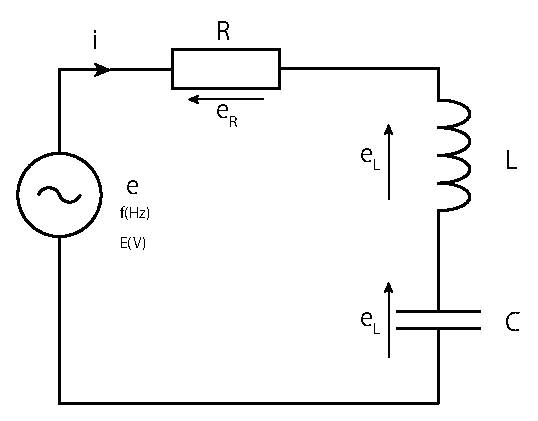
\includegraphics[clip, width=0.35\columnwidth]{img/1a.eps}
 \caption{RLC直列回路}
}
\end{figure}

いま回路に流れる電流を、$i=\sqrt{2}I\sin \omega t$と仮定すると

\begin{eqnarray}
\left\{\vbox to 24pt{} \begin{array}{ll}
e_{R}&=\sqrt{2} RI\sin \omega t\\
e_{L}&=\sqrt{2}\omega LI \sin \biggl( \omega t+\dfrac{\pi}{2}\biggr)\\
e_{C}&=\sqrt{2}\frac{1}{\omega C}I \sin \biggl( \omega t-\dfrac{\pi}{2}\biggr)\\
e&=e_{R}+e_{L}+e_{C}=\sqrt{2}E\sin (\omega t + \theta)
\end{array} \right.
\end{eqnarray}

これらをベクトル図に示した物が図\ref{fig:1b}である。
\begin{figure}[h]
\label{fig:1b}
\center{
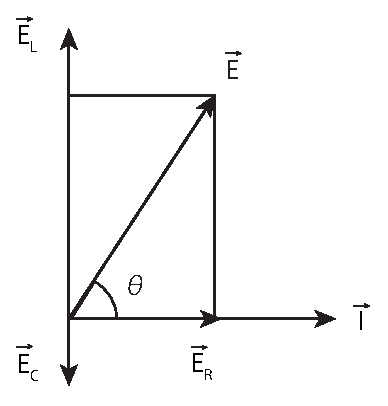
\includegraphics[clip, width=0.35\columnwidth]{img/1b.eps}
\caption{ベクトル図}
}
\end{figure}
これより
\begin{align}
&E^{2}={E_{R}}^{2}+(E_{L}-E{C})^{2}=\Biggl\{R^{2}+\biggl(\omega L-\frac{1}{\omega C}\biggr)^{2}\Biggr\}I^{2}=Z^{2}I^{2}\nonumber\\
&\therefore E=ZI=\Biggl\{R^{2}+\biggl(\omega L-\frac{1}{\omega C}\biggr)^{2}\Biggr\}^{\frac{1}{2}}I
\end{align}
また
\begin{eqnarray}
\theta &=\tan ^{-1}\frac{E_{L}-E{C}}{E_{R}}=\tan ^{-1}\frac{\omega L-\dfrac{1}{\omega C}}{R}
\end{eqnarray}
ところで図\ref{fig:1a}の回路においてリアクタンス成分が0になる条件を直列共振条件という。
このときは
\begin{align}
&\omega _{0}L-\frac{1}{\omega _{0}C}=0\\
&\omega_{0}=\frac{1}{\sqrt{LC}}\\
&Z_{0}=R\\
&I_{0}=\frac{E}{R}\\
&\theta =\tan^{-1}0=0^\circ
\end{align}
が成立し、インピーダンス$Z$は最小に、電流は最大に、また位相角$\theta$は0となる。
また、このとき
\begin{align}
\left\{\vbox to 24pt{} \begin{array}{ll}
E_{R0}&=RI_{0}=R\times\dfrac{E}{R}=E\\
E_{C0}&=\dfrac{1}{\omega_{0}C}I_{0}=\dfrac{E}{\omega_{0}CR}\\
E_{L0}&=\omega_{0}LI_{0}=\omega_{0}L\times\dfrac{E}{R}
\end{array} \right.
\end{align}
となる。
いま電源周波数$f$を変化したときの$I,\ Z,\ \theta,\ $の変化を図\ref{fig:2}に模式的に示す。
図よりわかるように、直列共振回路は特定の周波数成分の信号を取り出すときに使用される。
以上の性質を実験によって確かめることとする。
\begin{figure}[htbp]
 \centering
 \subfigure[電流の変化]{
  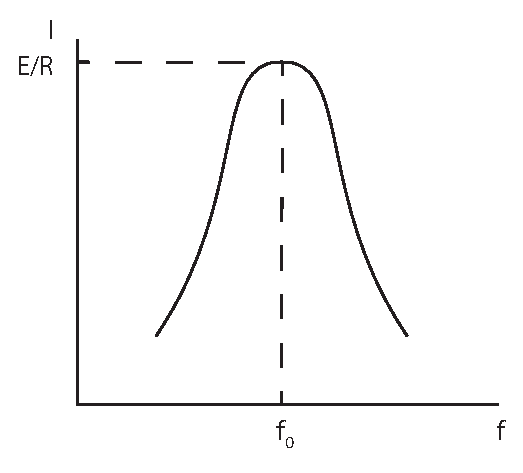
\includegraphics[clip, width=0.3\columnwidth]{img/2a.eps}
  \label{fig:2a}}
 \subfigure[インピーダンスの変化]{
  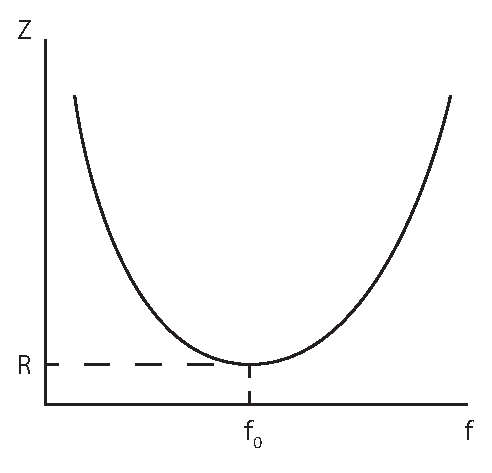
\includegraphics[clip, width=0.3\columnwidth]{img/2b.eps}
  \label{fig:2b}}
 \subfigure[位相の変化]{
  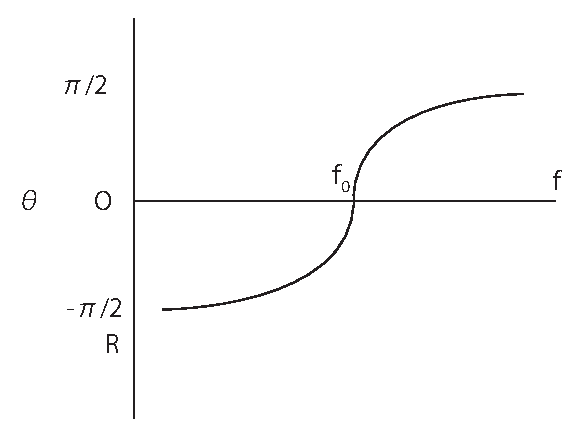
\includegraphics[clip, width=0.3\columnwidth]{img/2c.eps}
  \label{fig:2c}}
 \caption{直列共振回路の特性}
 \label{fig:2}
\end{figure}

%
\section{実験方法}

実験回路を図\ref{fig:3}に示す。
回路素子部分をブレッドボード上に結線し交流電源として発信器を用いる。
発信器の出力側にオシロスコープのCH1側を接続し、抵抗RにCH2側を接続して波形を観測から実験値を読み取る。
また、適宜デジタルマルチメータを用いて各素子の電圧を観測する。
\begin{figure}[h]
\label{fig:3}
\center{
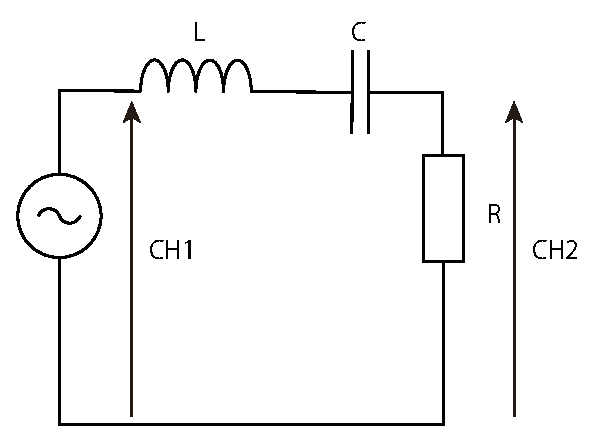
\includegraphics[clip, width=0.35\columnwidth]{img/3.eps}
\caption{実験回路図}
}
\end{figure}

\subsection{実験1 周波数特性}
(1)実験回路を結線して発振器出力を常に一定に保ちながら周波数を500 Hz~100 kHzまで変化させて各素子の電圧を測定し、周波数に対する電流の特性を測定する、
特に、電流が最大となる今日進展はより細かく測定する。
($R=1\ \si{[k\ohm]}, C=47\ \si{[nF]}, 発振器出力=1\ \si{[V]}$)

(2)抵抗値を変えて(1)の実験を行う。
ただし、束帯電圧は抵抗Rのみとする。
\subsection{実験2 静電容量依存性}
周波数を固定して回路の静電容量を変化させ、制電少量に対する電流の特性を測定する。
コンデンサCの値は$0.001\ \si{\micro F}~0.2\ \si{\micro F}$まで変化させて測定を行う。
($f=11\ \si{[kHz]}, 出力=1\ \si{[V]}, R=1\ \si{[k\ohm]},$Lは(1)で用いた物、抵抗の電圧を測定し、$I=|V_{R}|/R$とする。)
\subsection{実験3 $r_{L}$の測定}
コイルの束帯分$r_{L}$をマルチメータを使って測定する。
以後、コイルの抵抗としては、この値を使用する。

\subsection{使用器具}
この実験で使用した器具を表\ref{cal:item}に示す。
\begin{table}[!h]
\centering
\caption{使用器具}
\label{cal:item}
\begin{tabular}{|l|l|l|l|}
\hline
\multicolumn{1}{|c|}{器具名} & メーカ名    & 型番      & シリアルナンバー   \\ \hline
デュアルディスプレイマルチメータ          & TEXIO   & DL-2040 & 13020563   \\ \hline
デュアルディスプレイマルチメータ          & TEXIO   & DL-2040 & 130205538  \\ \hline
発信器                       & KENWOOD & AG-2040 & 6050017    \\ \hline
可変コンデンサ                   & HP      & 4440B   & 1224J04420 \\ \hline
\end{tabular}
\end{table}
%
\section{実験結果}
\subsection{実験1の結果}
実験1(1)、(2)の結果を表\ref{cal:result1(1)}、\ref{cal:result1(2)}に示す。
\begin{table}[!h]
\centering
\caption{実験1(1)の結果}
\label{cal:result1(1)}
\begin{tabular}{|l|l|l|l|}
\hline
周波数 {[}kHz{]} & Rにかかる電圧 {[}V{]} & Cにかかる電圧 {[}V{]} & Lにかかる電圧 {[}V{]} \\ \hline \hline
0.5           & 0.1561          & 0.98            & 0.0177          \\ \hline
0.6           & 0.1852          & 0.955           & 0.0237          \\ \hline
0.8           & 0.2524          & 0.998           & 0.0404          \\ \hline
1             & 0.3244          & 0.995           & 0.0651          \\ \hline
2             & 0.635           & 0.975           & 0.2474          \\ \hline
3             & 0.863           & 0.896           & 0.496           \\ \hline
3.5           & 0.922           & 0.828           & 0.612           \\ \hline
4             & 0.946           & 0.716           & 0.746           \\ \hline
4.5           & 0.941           & 0.663           & 0.796           \\ \hline
5             & 0.897           & 0.552           & 0.87            \\ \hline
6             & 0.825           & 0.4315          & 0.943           \\ \hline
8             & 0.648           & 0.253           & 0.994           \\ \hline
10            & 0.521           & 0.162           & 1.007           \\ \hline
20            & 0.2631          & 0.0417          & 1.016           \\ \hline
30            & 0.1722          & 0.0181          & 1.004           \\ \hline
40            & 0.1284          & 0.0095          & 1.005           \\ \hline
50            & 0.1025          & 0.0045          & 1.004           \\ \hline
60            & 0.0844          & 0.0018          & 1.007           \\ \hline
80            & 0.061           & 0               & 1.011           \\ \hline
100           & 0.0464          & 0               & 1.004           \\ \hline
\end{tabular}
\end{table}

\begin{table}[!h]
\centering
\caption{実験1(2)の結果}
\label{cal:result1(2)}
\begin{tabular}{|l|l|}
\hline
周波数{[}kHz{]} & Rの電圧 {[}V{]} \\ \hline \hline
0.5          & 0.3119       \\ \hline
0.6          & 0.3564       \\ \hline
0.8          & 0.4625       \\ \hline
1            & 0.573        \\ \hline
2            & 0.845        \\ \hline
3            & 0.947        \\ \hline
3.5          & 0.976        \\ \hline
4            & 0.978        \\ \hline
4.5          & 0.975        \\ \hline
5            & 0.970        \\ \hline
6            & 0.938        \\ \hline
8            & 0.866        \\ \hline
10           & 0.775        \\ \hline
20           & 0.481        \\ \hline
30           & 0.33         \\ \hline
40           & 0.257        \\ \hline
50           & 0.0248       \\ \hline
60           & 0.1706       \\ \hline
80           & 0.1235       \\ \hline
100          & 0.0908       \\ \hline
\end{tabular}
\end{table}

\subsection{実験2の結果}
実験2の結果を表\ref{cal:result2}に示す。
\begin{table}[!h]
\centering
\caption{実験2の結果}
\label{cal:result2}
\begin{tabular}{|l|l|}
\hline
コンデンサ{[}pF{]} & Rの電圧 {[}V{]} \\ \hline
1             & 0.0819       \\ \hline
2             & 0.1942       \\ \hline
3             & 0.3483       \\ \hline
4             & 0.549        \\ \hline
5             & 0.768        \\ \hline
6             & 0.914        \\ \hline
7             & 0.947        \\ \hline
8             & 0.91         \\ \hline
9             & 0.852        \\ \hline
10            & 0.801        \\ \hline
20            & 0.575        \\ \hline
30            & 0.517        \\ \hline
40            & 0.492        \\ \hline
50            & 0.477        \\ \hline
60            & 0.4661       \\ \hline
70            & 0.4614       \\ \hline
80            & 0.4512       \\ \hline
90            & 0.4532       \\ \hline
100           & 0.4511       \\ \hline
150           & 0.4406       \\ \hline
200           & 0.4372       \\ \hline
\end{tabular}
\end{table}
\subsection{実験3の結果}
実験3の結果を表\ref{cal:result3}に示す。
\begin{table}[!h]
\centering
\caption{実験3の結果}
\label{cal:result3}
\begin{tabular}{|l|}
\hline
コイルの抵抗分 {[}Ω{]}            \\ \hline
\multicolumn{1}{|r|}{49.9} \\ \hline
\end{tabular}
\end{table}
\clearpage

\section{結果の整理}
\subsection{周波数特性}
以下の式より周波数に対する電流特性を図\ref{fig:f-I}に示す。
\begin{align}
I&=\frac{e_{R}}{R}
\end{align}

\begin{figure}[!h]
\center{
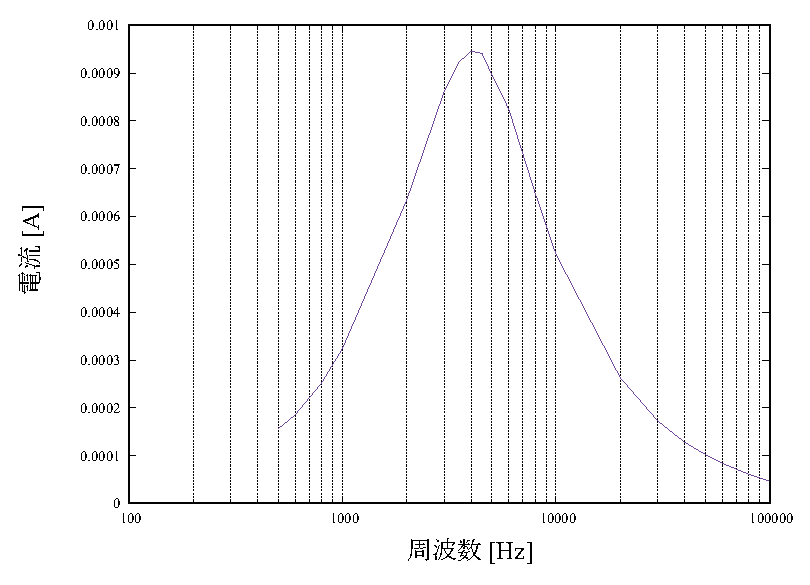
\includegraphics[clip, width=0.7\columnwidth]{img/f-I.eps}
\caption{周波数に対する電流特性}
\label{fig:f-I}
}
\end{figure}

また以下の式より周波数に対するインピーダンス特性を図\ref{fig:f-z}に示す。
\begin{align}
Z&=\frac{e}{I}\\
\end{align}

\begin{figure}[H]
\center{
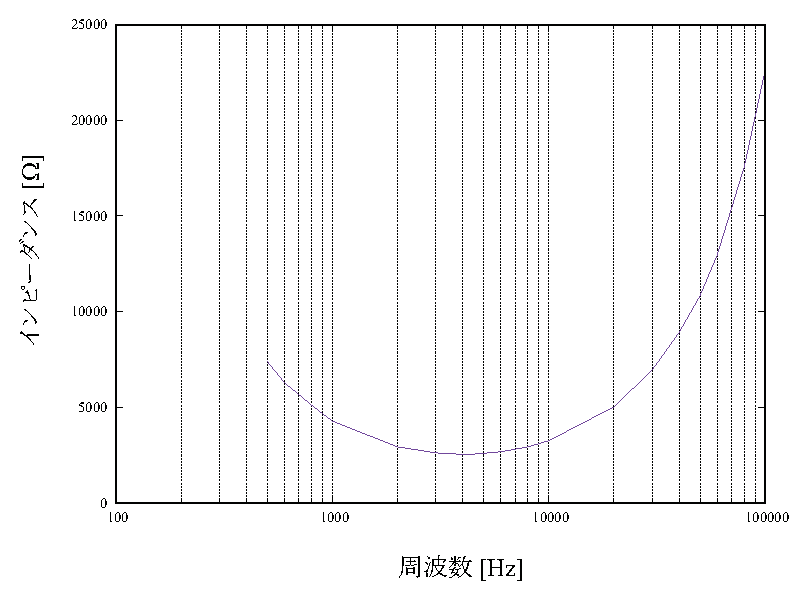
\includegraphics[clip, width=0.7\columnwidth]{img/f-z.eps}
\caption{周波数に対するインピーダンス特性}
\label{fig:f-z}
}
\end{figure}

ここで共振周波数$f_{0}$について考える。
図\ref{fig:f-I}より電流が最大になる周波数が最大周波数と考えられるので、
\begin{align}
f_{0}&=4000\ \si{Hz}
\end{align}

これよりLの値が求められる。
\begin{align}{
&2\pi f_{0}L=\frac{1}{2\pi f_{0}C}\nonumber\\
&L=33.7\ \si{mH}\nonumber
}\end{align}

これらの値と以下の式を用いて周波数に対する位相特性を図\ref{fig:f-theta}に示す。
\begin{align}
\theta&=\tan^{-1}\frac{\omega L-\frac{1}{\omega C}}{R+R_{L}}
\end{align}

\begin{figure}[H]
\center{
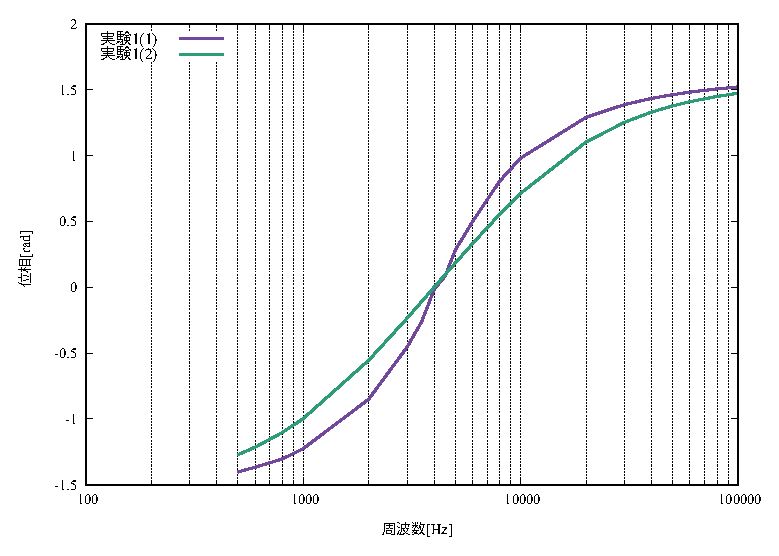
\includegraphics[clip, width=0.7\columnwidth]{img/f-theta.eps}
\caption{周波数に対する位相特性}
\label{fig:f-theta}
}
\end{figure}

Lの値が分かったことにより電流の計算値$I_{math}$が求められる。
以下の式より電流の値を求めた上で周波数に対する電流特性を図\ref{fig:f-Imath}に示す。

\begin{align}
I_{math}&=\frac{V}{\sqrt{(R+r_{L})^2+(2\pi f_{0}L-\frac{1}{2\pi f_{0}})^2}}
\end{align}

\begin{figure}[H]
\center{
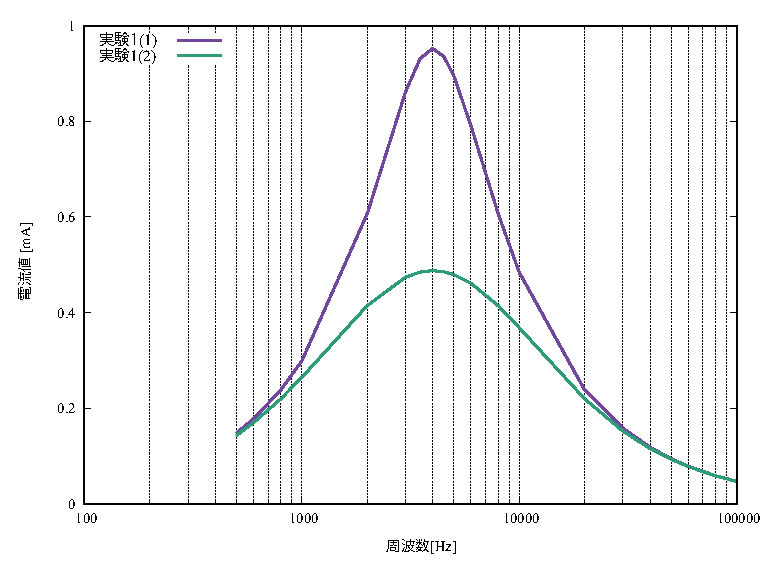
\includegraphics[clip, width=0.7\columnwidth]{img/f-Imath.eps}
\caption{周波数に対する電流特性(計算によって求めた値を使用)}
\label{fig:f-Imath}
}
\end{figure}

また(i)$f<f_{0}$, (ii)$f=f_{0}$, (iii)$f>f_{0}$のときについて回路の状態をベクトル図で表現する。

\begin{figure}[H]
\center{
\subfigure[(i) f<$f_{0}$の場合]{
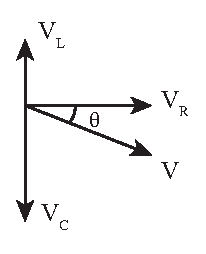
\includegraphics[clip, width=0.25\columnwidth]{img/ff0.eps}
}
\subfigure[(ii) f=$f_{0}$の場合]{
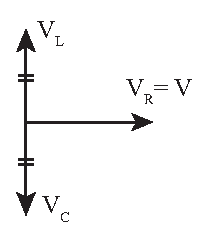
\includegraphics[clip, width=0.25\columnwidth]{img/f0.eps}
}
\subfigure[(iii) f>$f_{0}$の場合]{
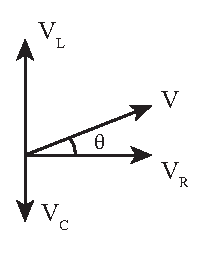
\includegraphics[clip, width=0.25\columnwidth]{img/f0f.eps}
}}\end{figure}

また回路の先鋭度を求める。
実験1の先鋭度を$Q_{1}$、$Q_{2}$とする。
\begin{align}
Q_{1}&=\frac{1}{2\pi f_{0}RC}\nonumber\\
&=0.847\\
Q_{2}&=0.423\
\end{align}
\subsection{C依存性}
実験3より静電容量に対する電流特性を図\ref{fig:c-I}に示す。
\begin{figure}[H]
\center{
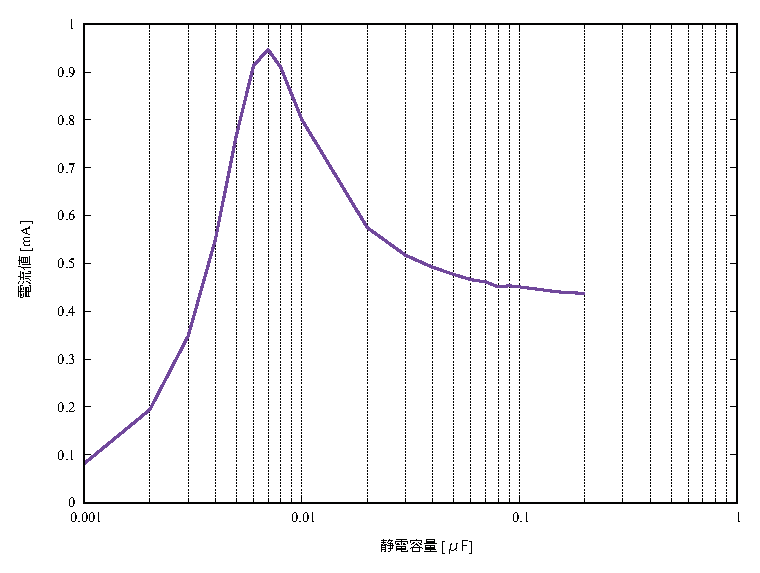
\includegraphics[clip, width=0.7\columnwidth]{img/c-I.eps}
\caption{静電容量に対する電流特性}
\label{fig:c-I}
}\end{figure}
%
\section{調査事項}
%
\end{document}